\section{Tapatybės atributų valdymo modelis} \label{section:BCIDM}

Atsižvelgus į blokų grandinės savybes, tinkamas tapatybės valdymo problemoms spręsti, šiame skyriuje pateikiamas
vieša blokų grandine paremtas skaitmeninės tapatybės valdymo modelis. Modelis skirtas spręsti\hypertarget{IDM:problemsSummarized}{~\ref{IDM:problemsSummarized}} skyrelyje
apibendrintoms naudotojų problemoms. Kadangi tapatybės valdymas apima
daug skirtingų procesų, aprašomas modelis apsiriboja asmens tapatybės atributų valdymu, saugojimu ir perdavimu.

Modelio architektūra kurta atsižvelgiant į MIT tyrime \cite{MITPaper} pristatytus teorinius protokolus, kurie apibrėžia
mobiliųjų programėlių, naudotojo bei blokų grandinės bendravimą, asmeniui suteikiant telefone saugomą
informaciją (pvz. lokacijos duomenis) naujai parsisiųstai programėlei. Aprašomas modelis modifikuoja bendravimą, siekiant 
jį pritaikyti naudojimui internete, taip pat išplečia funkcionalumą, leidžiant naudotojui pačiam įvesti norimą informaciją.

\subsection{Reikalavimai} \label{BCIDM:requirements}

Naudotojams kylančios problemos tapatybės valdyme remiasi į tai, kad jų tapatybė yra
visiškai patikėta valdyti tapatybės tiekėjams. Dėl menko naudotojų įsitraukimo į tapatybės valdymo
procesus, asmenys neretai lieka tik pasyvūs stebėtojai.

Siekiant išspręsti šią problemą, kuriamo modelio reikalavimai kurti pagal į naudotoją orientuotos tapatybės
(angl. \textit{user-centric identity}) principus. Ši paradigma akcentuoja naudotojus kaip centrinę
identiteto valdymo sistemų dalį, perduodant paslaugų ir tapatybės tiekėjų turimą tapatybės kontrolę
naudotojams \cite{Cao2010}. Tokiu būdu, naudotojai turi aktyviau prižiūrėti ir dalyvauti tapatybės
valdymo procesuose (dažniausiai naudojant papildomą programinę įrangą),
tačiau geriau žino, kaip ir kur yra naudojami jų asmens duomenys.

Taikant į asmenis orientuotos skaitmeninės tapatybės principus, reikalavimai modeliui suformuluoti naudotojų istorijų forma:

\begin{enumerate}
    \item Kaip interneto naudotojas, aš noriu žinoti, kurios programos turi prieigą prie kurių mano asmens duomenų.
    \item Kaip interneto naudotojas, aš noriu kontroliuoti savo asmens duomenis ir pats pasirinkti, kurios mano naudojamos paslaugos gali pasiekti mano
    asmens duomenis.
    \item Kaip interneto naudotojas, aš noriu galimybės lengvai atnaujinti savo asmens duomenis vienoje vietoje.
    \item Kaip interneto naudotojas, aš nenoriu, jog mano asmens duomenų pasiekiamumas priklausytų tik nuo vienos trečiosios šalies pasiekiamumo.
\end{enumerate}

Pateiktos naudotojų istorijos padengia 1 skyriuje apibrėžtus asmenų poreikius tapatybės valdymo
sistemoms bei išskirtas kontrolės, pasitikėjimo ir skaidrumo trūkumo problemas. Interneto tapatybių valdymo sistemų saugumo atakos (angl.
\textit{cross site scripting}, \textit{phishing}) yra plati tema, verta atskiro tyrimo, tad ji šiame modelyje nebus nagrinėjama.

\subsection{Modelio dalys}

Modelis sudarytas iš trijų dalių: atributų saugyklos išmaniojo kontrakto, paslaugų registro išmaniojo kontrakto
bei atributų valdymo programos.

\subsubsection{Atributų saugyklos išmanusis kontraktas} \label{BCIDM:blockchainFunctions}

Atributų saugyklos išmaniajame kontrakte yra saugomi šifruoti naudotojų atributai bei jų suteikimo logika. Šis kontraktas atsakingas už:

\begin{itemize}
    \item naudotojo atliekamą prieigų suteikimą. Naudotojas, kviesdamas kontrakto funkciją, gali pasirinkti,
    ar suteikti konkrečiai paslaugai prieigą prie jos norimo atributo. Prieigos yra valdomos ne visos tapatybės, o
    atskirų atributų lygmenyje;

    \item šifruotų atributų saugojimą. Kontrakte saugomi naudotojo tapatybės atributai. Kadangi modelyje naudojama vieša blokų
    grandinė, joje esantys duomenys prieinami visiems - dėl to saugomi šifruoti atributai. Jeigu naudotojas N
    yra autorizavęs paslaugą P pasiekti atributą A, tuomet kontrakte išsaugomas N ir P simetrišku šifro raktu (angl.
    \textit{symmetric encryption key}) užšifruotas atributas A. Taip tik paslauga P
    ir naudotojas N, turintys šifro raktus, galės perskaityti viešame išmaniajame kontrakte esantį atributą;

    \item pateikiamas funkcijas paslaugoms bei naudotojui pasiekti atributus. Išmanusis kontraktas pirmiausia atsižvelgia
    į funkcijos kvietėją. Jei kreipiasi naudotojas, jam grąžinama šifruota atributo reikšmė. Jei kreipiasi paslauga, tikrinama,
    ar naudotojas yra patvirtinęs jos prieigą norimam atributui. Jei taip, grąžinama šifruota reikšmė. Jei ne, grąžinamas pranešimas,
    kad prieiga atmesta. Jeigu naudotojas šios paslaugos prieigos dar nesvarstęs, apie paslaugos P siekį gauti naudotojo N atributą A
    pranešama naudotojui. Kai jis prieigą patvirtins arba atmes, paslauga galės pasiekti atributą A.
\end{itemize}

\subsubsection{Atributų valdymo programa}

Atributų valdymo programa yra skirta palengvinti naudotojo bendravimą su blokų grandine. Teoriškai, naudotojas galėtų pats formuoti užklausas,
generuoti šifro raktus, perduoti jos paslaugoms, užšifruoti ir dešifruoti siunčiamas reikšmes, tačiau tai nėra patogu. Dėl to ši
programa padeda atlikti \enquote{nematomą darbą} bei supaprastina naudotojo sąsają su bloko grandine. Programoje naudotojas gali:

\begin{itemize}
    \item suteikti arba atmesti paslaugai P prieigą prie atributo A,
    \item peržvelgti suteiktas prieigas ir keisti jas,
    \item įvesti, keisti ar trinti atributų reikšmes.
\end{itemize}

Atributų valdymo programos veikimas panašus į kriptovaliutos piniginės veikimą. Kaip tokia piniginė leidžia naudotojui per vartotojo sąsają
pervesti pinigus iš naudotojo sąskaitos į kitą sąskaitą, taip atributų valdymo programa leidžia naudotojui
valdyti savo paskyros atributus blokų grandinės išmaniajame kontrakte. Programa veikia naudotojo vardu (angl. \textit{on user's behalf}),
turėdama jo privatų raktą
- taip ji gali kreiptis į blokų grandinę
iš naudotojo paskyros, o išmanusis kontraktas, gavęs užklausą iš atributų valdymo programos,
žino, koks naudotojas kreipiasi į funkciją.

Modelyje nėra apibrėžiama, kaip turi būti įgyvendinta ši programa - tai gali būti kompiuterio darbalaukio programa,
mobilioji programėlė ar interneto tinklapis. 

\subsubsection{Paslaugų registro išmanusis kontraktas} \label{BCIDM:serviceRegister}

Šiame modelyje paslaugos yra identifikuojamos pagal jų blokų grandinės paskyros adresą. Atributų valdymo programa,
skaitanti išmaniajame kontrakte laukiančias užklausas, jose mato išsaugotą besikreipusios paslaugos adresą.

Nors adresas yra viešas ir unikaliai identifikuoja kiekvieną blokų grandinės dalyvį, turintį paskyrą, tačiau iš adreso nustatyti tikrąją dalyvio tapatybę yra sudėtinga -
pats adresas nėra tiesiogiai susiejamas su tikru asmens identifikatoriumi (pvz. asmens kodu ar paslaugos įmonės kodu).
Tokiu būdu, atributų valdymo programoje matant tik paslaugos adresą dalyvis gali nežinoti, kokią paslaugą jis autorizuoja.

Šiai problemai spręsti modelyje yra atskiras išmanusis kontraktas, kuris funkcionuoja kaip paslaugų registras. Kiekviena
paslauga, besinaudojanti modeliu, atlieka vieną transakciją į šį registrą, joje nusiųsdama savo pavadinimą bei slaptą kodą,
suteiktą naudotojo arba sugeneruotą atributų valdymo programos. Kai atributų saugyklos kontrakte bus išsaugota nauja paslaugos
P užklausa pasiekti atributą, atributų valdymo programa pagal P viešą raktą gali kreiptis
į šį registrą ir įsitikinti, ar P tikrai užsiregistravo (rasti iš P paskyros atliktą transakciją) ir iš kodo
nuspręsti, ar tai tikrai yra paslauga, kuria asmuo naudojasi (taip užsiregistravę, bet kodo neturintys programišiai negali
apsimesti kita įmone). Atributų valdymo programa, remdamasi paslaugų registru, gali atfiltruoti ir naudotojui pateikti tik
validžias paslaugų užklausas.

Verta pastebėti, kad paslaugų registras nėra vienintelis įmanomas būdas autentifikuoti paslaugas. Galimos alternatyvos plačiau apžvelgiamos
modelio vertinimo \hypertarget{section:blockchainIDMevaluation}{skyriuje}.

\subsection{Pagrindiniai naudojimo atvejai}

Šiame skyriuje UML sekų diagramomis pateikiami pagrindiniai modelio panaudos atvejai (angl. \textit{use cases}).

\subsubsection{Naudotojo adreso suteikimas paslaugai}

Kai paslauga bei asmuo naudojasi aprašomu modeliu, paslauga paprašo naudotojo pateikti jo adresą (naudotojo patogumui, adresas rodomas
atributų valdymo programoje),
kuris yra viešas naudotojo identifikatorius blokų grandinėje.
Gavus šį adresą, paslauga iš atributų valdymo programos prašo šifro rakto, su kuriuo galės dešifruoti iš blokų grandinės gautus atributus.
Su gautu adresu paslauga P gali kreiptis į blokų grandinę ir prašyti norimų naudotojo atributų (žr.\hypertarget{fig:userGivesAddress}{~\ref{fig:userGivesAddress} pav.}).

Modelis neapibrėžia, kada naudotojas N privalo pateikti adresą paslaugai P. Svarbu, kad paslauga P gautų šį adresą ir unikalų šifro raktą tarp N ir P,
nes be jų P negalės gauti ir perskaityti norimų tapatybės duomenų. Šis suteikimas galėtų būti atliekamas prisijungimo metu, įtraukiant
papildomą žingsnį.

\begin{figure}[H]
    \centering
    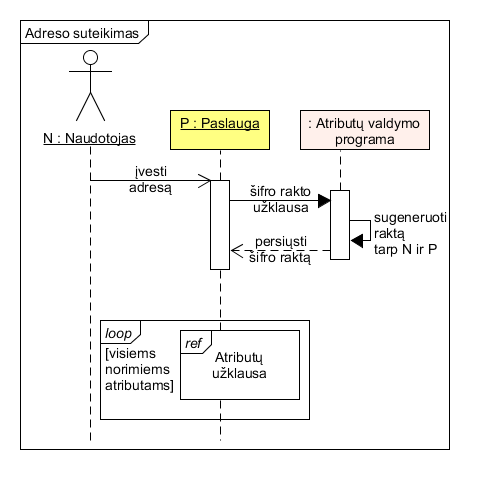
\includegraphics[scale=0.6]{img/userGivesAddress}
    \caption{Naudotojo adreso suteikimas paslaugai}
    \label{fig:userGivesAddress}
\end{figure}

\subsubsection{Paslaugos atliekama atributo užklausa} \label{BCIDM:askForAttribute}

Paslauga P, norinti gauti tam tikrą asmens atributą (pvz. gimimo datą)\footnote{ Paslaugai kreipiantis į kontraktą, ji turi žinoti, koks yra norimo atributo identifikatorius, kurį reikia perduoti į kontrakto funkciją. 
Atributų identifikatoriai gali būti pateikiami atskirame išmaniajame kontrakte arba kuriamo modelio interneto puslapyje.}
, kreipiasi į blokų grandinės išmanųjį kontraktą (žr.\hypertarget{fig:askForAttributeSequence}{~\ref{fig:askForAttributeSequence} pav.}).
Kontraktas tuomet patikrina, ar ši paslauga turi prieigą prie pageidaujamo atributo. Jei turi, tuomet grąžina šį atributą. Jis
užšifruotas paslaugos P turimu šifro raktu, tad paslauga gali jį dešifruoti ir perskaityti duomenis. Jei
naudotojas atmetęs prieigą, apie tai pranešama paslaugai. Jei naudotojas dar nesvarstęs šios prieigos, išsaugoma laukianti
(angl. \textit{pending}) paslaugos P atributo A užklausa ir laukiama naudotojo sprendimo. Naudotojas šią laukiančią užklausą galės pamatyti savo 
atributų valdymo programoje ir ten atlikti sprendimą.

\begin{figure}[h]
    \centering
    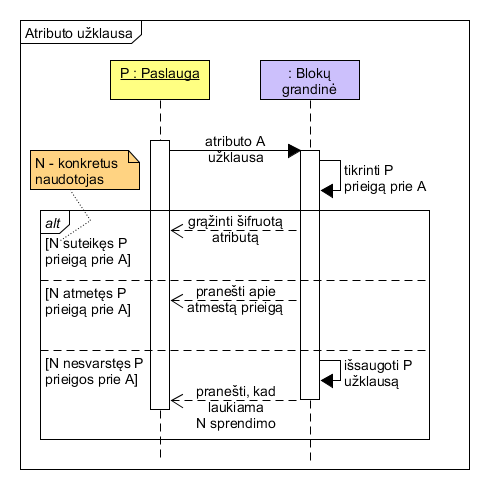
\includegraphics[scale=0.7]{img/askForAttributeSequence}
    \caption{Paslaugos atliekama atributo užklausa}
    \label{fig:askForAttributeSequence}
\end{figure}

\subsubsection{Naudotojo atliekamas paslaugos autorizavimas}

Atributų valdymo programa, stebinti išmaniuosiuose kontraktuose naujas paslaugų užklausas, praneša naudotojui apie dar
neatliktus autorizavimus. Tuomet naudotojas gali pasirinkti, ar suteikti, ar atmesti prieigą prie norimo atributo
A paslaugai P. (žr.\hypertarget{fig:givePermissions}{~\ref{fig:givePermissions} pav.}). Blokų grandinė asmeniui leidžia autorizuoti tik savo naudojamas paslaugas
\footnote{ Ar naudotojo N prieigai pakeisti siunčiamą žinutę tikrai siunčia N, blokų grandinė atskiria iš žinutės parašo.}.

Jei naudotojas prieigą suteikia, tuomet atributų valdymo programa užšifruoja atributą A. Tai
daroma todėl, kad kiekvienas atributas, suteiktas paslaugai P, turi būti užšifruotas tik paslaugai P ir naudotojui N
žinomu šifro raktu bei nusiųstas
į išmanųjį kontraktą. Pati atributo reikšmė yra iš anksto įvesta naudotojo į atributų valdymo programą.
Užšifravus reikšmę, duomenys nusiunčiami į išmanųjį kontraktą ir jame pažymima, kad paslauga P autorizuota
pasiekti atributą A.

Jei naudotojas prieigą atmeta, tuomet blokų grandinėje pažymima, kad paslauga P nėra autorizuota pasiekti atributą A.

Jei naudotojas vėliau nuspręstų pakeisti savo sprendimą (pvz. panaikinti suteiktas prieigas prie atributo A paslaugai P),
jis šį paslaugos autorizavimo procesą galėtų pakartoti ir jau esamai prieigai.


\begin{figure}[h]
    \centering
    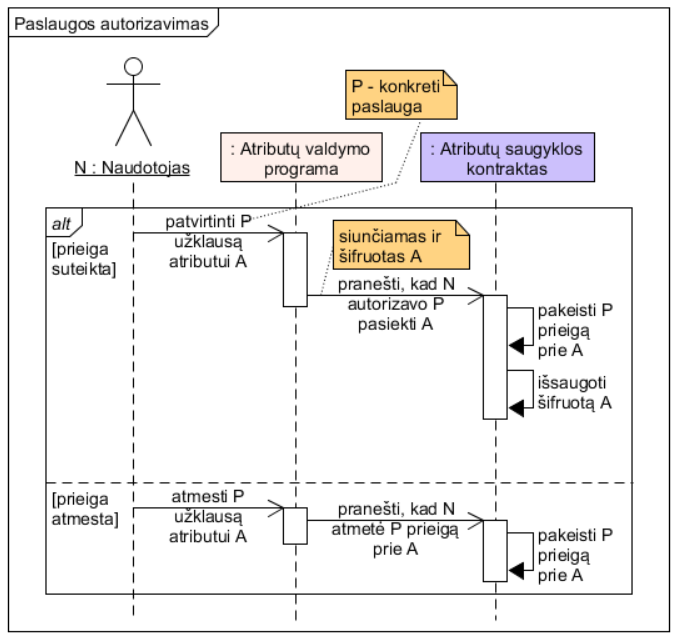
\includegraphics[scale=0.65]{img/givePermissions}
    \caption{Naudotojo atliekamas paslaugos autorizavimas}
    \label{fig:givePermissions}
\end{figure}

\subsubsection{Atributų valdymo programos atliekamas blokų grandinės stebėjimas} \label{BCIDM:blockchainMonitoring}

Blokų grandinės išmanusis kontraktas negali tiesiogiai pranešti išorinei (ne išmaniajame kontrakte esančiai) programai
apie įvykusius pasikeitimus. Todėl išmanusis kontraktas gali saugoti būseną, o ją vėliau pasiekia norinti taikomoji programa.
Tokiu būdu atributų valdymo programa periodiškai kreipiasi į išmanųjį kontraktą ir žiūri, ar yra naujų paslaugų užklausų. Jeigu jų yra,
atributų valdymo programa išsaugo pranešimą apie tai naudotojui (žr.\hypertarget{fig:checkForPendingPermissions}{~\ref{fig:checkForPendingPermissions} pav.}).\\
Panašiu stebėjimo principu pasikeitimus išmaniojo kontrakto būsenoje gali stebėti ir paslaugų tiekėjai
(pvz. apie pasikeitusias prieigas).

\begin{figure}[h]
    \centering
    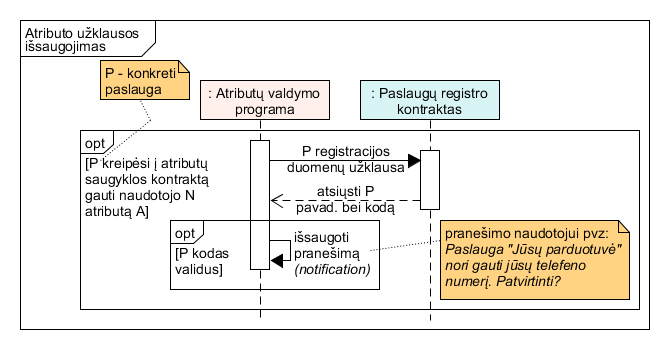
\includegraphics[scale=0.6]{img/checkForPendingPermissions}
    \caption{Atributų valdymo programos atliekamas blokų grandinės stebėjimas}
    \label{fig:checkForPendingPermissions}
\end{figure}